% answers.tex —— 1977 年·湖北卷 · 参考答案与详细解析片段
% 由 tools/generate_projects.py 依来源总账自 1977/1977_数学真题_湖北_试题.md + 1977/1977_数学真题_湖北_解析正文.md + 1977/1977_数学真题_湖北_答案要点.md 生成，勿手改（改源 MD 后重跑）


\begin{gktip}
固定源是题面与解答连续出现的《湖北1977年高考数学试题解》。下文逐题对照源解答并重新计算关键结论；原卷大题的汉字编号（一、二、三、四、五）已对应为第 1—5 题，第一题的（1）—（8）小题编号不变；参考题三题不计入考分，解析附于最后。源卷排印中把对数底数印作大写 Log、自然对数印作大写 Ln、正切印作 tg，本文按现代习惯分别记作小写 log、ln 与 tan，不影响数值。
\end{gktip}

\begin{answer}
\gksolhead{1}{}

\textbf{题目}（每小题 5 分，共 40 分）：

计算：

（1） $\sqrt{(-3)^2}$；$\sqrt[3]{(-27)^3}$．

（2） $\log_2 2+\log_5 1-\log_{\frac13}\frac{1}{27}$．

（3） $\left(\sqrt{\dfrac23}\right)^3\cdot\sqrt[3]{\left(\dfrac32\right)^2}\cdot\left(\dfrac23\right)^{-\frac56}$．

（4） 解方程：$x-\sqrt{8-x^2}=0$．

（5） 当 $m\leqslant 1$ 时，计算 $\sqrt{(m-1)^2}$．

（6） 求函数 $y=\dfrac{\sqrt{2-x}}{x+4}$ 的定义域．

（7） 分解因式：$x^4+x^2y^2+y^4$．

（8） 证明：$\operatorname{tg}22^\circ30'=\sqrt2-1$（不查表）．

\Needspace{4\baselineskip}
\textbf{解析}

\gksubpart{（1）}

\Needspace{5\baselineskip}
由 $(-3)^2=3^2$，得 $\sqrt{(-3)^2}=3$；又 $(-27)^3=-27$，且负数有唯一的奇次方根，故

\nopagebreak[4]
\[
\sqrt{(-3)^2}=3,
\qquad
\sqrt[3]{(-27)^3}=-27.
\]

\gksubpart{（2）}

\Needspace{5\baselineskip}
$\log_2 2=1$，$\log_5 1=0$；又

\nopagebreak[4]
\[
\log_{\frac13}\frac{1}{27}
=\log_{\frac13}\left(\frac13\right)^{3}=3,
\]

故原式 $=1+0-3=-2$。

\gksubpart{（3）}

\Needspace{5\baselineskip}
三个因子分别化成六次根式：

\nopagebreak[4]
\[
\begin{aligned}
\left(\sqrt{\frac23}\right)^{3}
&=\left(\frac23\right)^{\frac36}
=\sqrt[6]{\left(\frac23\right)^{9}},\\
\sqrt[3]{\left(\frac32\right)^{2}}
&=\left(\frac32\right)^{\frac46}
=\sqrt[6]{\left(\frac32\right)^{4}},\\
\left(\frac23\right)^{-\frac56}
&=\left(\frac32\right)^{\frac56}
=\sqrt[6]{\left(\frac32\right)^{5}}.
\end{aligned}
\]

\Needspace{5\baselineskip}
三者的乘积为

\nopagebreak[4]
\[
\sqrt[6]{\left(\frac23\right)^{9}\left(\frac32\right)^{9}}
=\sqrt[6]{\left[\left(\frac23\right)\left(\frac32\right)\right]^{9}}
=1.
\]

\gksubpart{（4）}

\Needspace{5\baselineskip}
移项得 $x=\sqrt{8-x^2}$，此时须 $x\geqslant 0$。两边平方：

\nopagebreak[4]
\[
x^2=8-x^2,
\qquad
x^2=4,
\qquad
x=\pm2.
\]

代入检验，$x=-2$ 使原方程左端为 $-4$，不适合原方程，是增根舍去；$x=2$ 满足原方程。故原方程的解为 $x=2$。

\gksubpart{（5）}

\Needspace{5\baselineskip}
由 $m\leqslant 1$ 得 $m-1\leqslant 0$，故

\nopagebreak[4]
\[
\sqrt{(m-1)^2}=|m-1|=-(m-1)=1-m.
\]

\gksubpart{（6）}

\Needspace{5\baselineskip}
要使函数有意义，须

\nopagebreak[4]
\[
\begin{cases}
2-x\geqslant 0,\\
x+4\ne0.
\end{cases}
\]

即 $x\leqslant 2$ 且 $x\ne-4$。因此定义域为 $-4<x\leqslant 2$ 或 $x<-4$ 的实数（即 $x\leqslant 2$ 且 $x\ne-4$）。

\gksubpart{（7）}

\Needspace{5\baselineskip}
先用平方差配立方：注意 $x^4+x^2y^2+y^4=(x^2+y^2)^2-x^2y^2$，故

\nopagebreak[4]
\[
x^4+x^2y^2+y^4
=(x^2+y^2-xy)(x^2+y^2+xy).
\]

在有理式范围内不能再分。

\gksubpart{（8）}

\Needspace{5\baselineskip}
由半角公式，

\nopagebreak[4]
\[
\operatorname{tg}\frac{45^\circ}{2}
=\frac{1-\cos45^\circ}{\sin45^\circ}.
\]

\Needspace{5\baselineskip}
以 $\cos45^\circ=\sin45^\circ=\dfrac{\sqrt2}{2}$ 代入：

\nopagebreak[4]
\[
\begin{aligned}
\operatorname{tg}22^\circ30'
&=\frac{1-\dfrac{\sqrt2}{2}}{\dfrac{\sqrt2}{2}}
=\frac{2-\sqrt2}{\sqrt2}
=\frac{(2-\sqrt2)\sqrt2}{2}\\
&=\frac{2\sqrt2-2}{2}
=\sqrt2-1.
\end{aligned}
\]

\gkanswer{答案（1）：$3$；$-27$。}

\gkanswer{答案（2）：$-2$。}

\gkanswer{答案（3）：$1$。}

\gkanswer{答案（4）：$x=2$。}

\gkanswer{答案（5）：$1-m$。}

\gkanswer{答案（6）：$-4<x\leqslant 2$ 或 $x<-4$（即 $x\leqslant 2$ 且 $x\ne-4$）。}

\gkanswer{答案（7）：$(x^2+y^2-xy)(x^2+y^2+xy)$。}

\gkanswer{答案（8）：见解析版}

\end{answer}
\begin{answer}
\gksolhead{2}{}

\textbf{题目}（10 分）：

围一矩形场地，一边利用房屋的墙，其他三边用 $L$ 米的篱笆围成，问怎样围才能使面积最大？最大面积是多少？

\begin{gktip}
原源 PDF 第 3 页附有矩形场地与房屋墙的示意图；LaTeX 版按源图重绘。
\end{gktip}
\nopagebreak[4]
\begin{center}% 1977 年湖北卷第二题：矩形场地一边靠房屋的墙（斜线段示墙），平行于墙的一边长标 x（按源卷第 3 页布局）
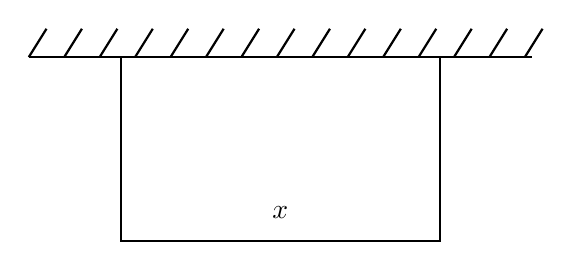
\begin{tikzpicture}[scale=0.9]
  \draw[thick] (0,0) rectangle (4.5,2.6);
  \draw[thick] (-1.3,2.6)--(5.8,2.6);
  \foreach \i in {0,...,14}
    \draw[thick] ({-1.3+0.5*\i},2.6) -- ({-1.05+0.5*\i},3.0);
  \node at (2.25,0.4) {$x$};
\end{tikzpicture}
\end{center}
\nopagebreak[4]
\Needspace{4\baselineskip}
\textbf{解析}

如图，设与墙平行的一边长为 $x$ 米，则与墙垂直的两边各长 $\dfrac{L-x}{2}$ 米（三边共用篱笆 $L$ 米）。这时矩形面积
\nopagebreak[4]
\begin{center}% 1977 年湖北卷第二题：矩形场地一边靠房屋的墙（斜线段示墙），平行于墙的一边长标 x（按源卷第 3 页布局）
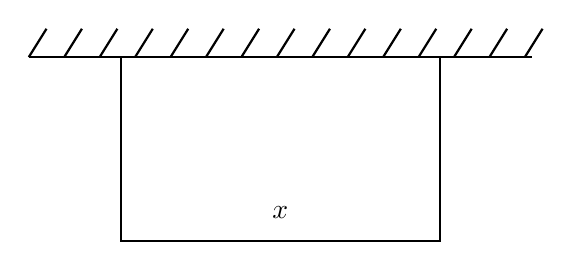
\begin{tikzpicture}[scale=0.9]
  \draw[thick] (0,0) rectangle (4.5,2.6);
  \draw[thick] (-1.3,2.6)--(5.8,2.6);
  \foreach \i in {0,...,14}
    \draw[thick] ({-1.3+0.5*\i},2.6) -- ({-1.05+0.5*\i},3.0);
  \node at (2.25,0.4) {$x$};
\end{tikzpicture}
\end{center}
\nopagebreak[4]
\nopagebreak[4]
\[
\begin{aligned}
S&=x\left(\frac{L-x}{2}\right)
=-\frac12x^2+\frac L2x\\
&=-\frac12\left(x-\frac L2\right)^2+\frac{L^2}{8}.
\end{aligned}
\]

所以当 $x=\dfrac L2$（米）时，$S$ 有最大值 $\dfrac{L^2}{8}$（平方米）。这时的宽为 $\dfrac{L-x}{2}=\dfrac L4$（米）。

\textbf{答}：当与墙平行的一边长为 $\dfrac L2$ 米，与墙垂直的两边分别长为 $\dfrac L4$ 米时，围成的矩形面积最大，最大面积为 $\dfrac{L^2}{8}$ 平方米。

\gkanswer{答案：与墙平行的一边长 $\dfrac{L}{2}$ 米、与墙垂直的两边各长 $\dfrac{L}{4}$ 米时，围成的矩形面积最大，最大面积为 $\dfrac{L^2}{8}$ 平方米。}

\end{answer}
\begin{answer}
\gksolhead{3}{}

\textbf{题目}（10 分）：

已知直线 $L_1$ 方程为 $x+y-1=0$ 和点 $A(-3,0)$．

（1） 求与直线 $L_1$ 垂直且通过 $A$ 的直线方程；

（2） 求点 $A$ 到直线 $L_1$ 的距离．

\Needspace{4\baselineskip}
\textbf{解析}

\gksubpart{（1）}

\Needspace{5\baselineskip}
直线 $L_1$：$x+y-1=0$ 的斜率为 $-1$，因此与它垂直的直线斜率为 $1$。根据点斜式，过 $A(-3,0)$ 的所求直线方程为

\nopagebreak[4]
\[
\frac{y-0}{x+3}=1,
\]

\Needspace{5\baselineskip}
即

\nopagebreak[4]
\[
x-y+3=0.
\]

\gksubpart{（2）}

\Needspace{5\baselineskip}
由点到直线的距离公式，

\nopagebreak[4]
\[
d=\frac{|-3+0-1|}{\sqrt{1+1}}
=\frac{4}{\sqrt2}
=2\sqrt2.
\]

\gkanswer{答案（1）：$x-y+3=0$。}

\gkanswer{答案（2）：$2\sqrt2$。}

\end{answer}
\begin{answer}
\gksolhead{4}{}

\textbf{题目}（20 分）：

\Needspace{5\baselineskip}
解方程组：

\nopagebreak[4]
\[
\begin{cases}
\operatorname{Log}_2 x-\operatorname{Log}_4 y=0,\\
y^2-13x^2+36=0.
\end{cases}
\]

\Needspace{4\baselineskip}
\textbf{解析}

\Needspace{5\baselineskip}
方程组中 $x$、$y$ 须为正数。由换底公式，$\log_4y=\dfrac{\lg y}{\lg 4}=\dfrac12\log_2y$，故第一式即

\nopagebreak[4]
\[
\log_2x-\frac12\log_2y=0,
\]

\Needspace{5\baselineskip}
于是

\nopagebreak[4]
\[
x=\sqrt{y}.
\]

\Needspace{5\baselineskip}
代入第二式，得

\nopagebreak[4]
\[
y^2-13y+36=0,
\qquad
(y-9)(y-4)=0,
\]

\nopagebreak[4]
\[
y_1=9,
\qquad
y_2=4.
\]

\Needspace{5\baselineskip}
把 $y_1=9$、$y_2=4$ 分别代回 $x=\sqrt y$，得 $x_1=3$、$x_2=2$。经检验，两组都满足原方程组。故原方程组的解为

\nopagebreak[4]
\[
\begin{cases}
x_1=3,\\
y_1=9,
\end{cases}
\qquad
\begin{cases}
x_2=2,\\
y_2=4.
\end{cases}
\]

\gkanswer{答案：$(x,y)=(3,9)$ 或 $(2,4)$。}

\end{answer}
\begin{answer}
\gksolhead{5}{}

\textbf{题目}（20 分）：

作函数 $y=\sqrt3\cos 2x+\sin 2x$ 的图象（要求写出作图步骤，并画出草图）．

\begin{gktip}
\textbf{参考题}（不计入考分，只供录取后参考）
\end{gktip}

\Needspace{5\baselineskip}
\textbf{参考题 1．} 求下列函数的导数：

\nopagebreak[4]
\[
y=\sin x;\qquad y=\mathrm e^{3x};\qquad y=\operatorname{Ln}x;\qquad f(t)=A\sin(\omega t+\varphi).
\]

\textbf{参考题 2．} 设函数 $f(x)=x^3-12x+10$．

（1）求 $f(x)$ 的极值点；

（2）求 $f(1)$，$f(2)$，$f(-3)$．

\Needspace{5\baselineskip}
\textbf{参考题 3．} 解方程：

\nopagebreak[4]
\[
\begin{cases}
y''+3y'-4y=0,\\
y\big|_{x=0}=0,\\
y'\big|_{x=0}=-10.
\end{cases}
\]

\Needspace{4\baselineskip}
\textbf{解析}

\Needspace{5\baselineskip}
先用辅助角化简：

\nopagebreak[4]
\[
\begin{aligned}
y&=\sqrt3\cos 2x+\sin 2x
=2\left(\frac{\sqrt3}{2}\cos 2x+\frac12\sin 2x\right)\\
&=2\left(\sin\frac{\pi}{3}\cos 2x+\cos\frac{\pi}{3}\sin 2x\right)
=2\sin\left(2x+\frac{\pi}{3}\right).
\end{aligned}
\]

所以这个函数的周期为 $\pi$，振幅为 $2$。列表取一个周期的五点：当 $x=-\dfrac{\pi}{6}$、$\dfrac{\pi}{12}$、$\dfrac{\pi}{3}$、$\dfrac{7\pi}{12}$、$\dfrac{5\pi}{6}$ 时，$y$ 依次为 $0$、$2$、$0$、$-2$、$0$。函数图象（一个周期）的草图如下：
\nopagebreak[4]
\begin{center}% 1977 年湖北卷第五题：y=√3cos2x+sin2x=2sin(2x+π/3) 一个周期的草图，横轴记 X，刻度以 π/12 为格（按源卷第 4 页布局）
\begin{tikzpicture}[x=2.2cm,y=0.85cm]
  \draw[->] (-1.35,0)--(2.95,0) node[below right]{$X$};
  \draw[->] (0,-2.9)--(0,3.1);
  \foreach \k in {-2,...,10}
    \draw ({\k*pi/12},-0.08)--({\k*pi/12},0.08);
  \foreach \h in {-2,-1,1,2}
    \draw (-0.05,\h)--(0.05,\h);
  \node[below left] at (0,0) {$0$};
  \node[left] at (0,2) {$2$};
  \node[left] at (0,1) {$1$};
  \node[left] at (0,-1) {$-1$};
  \node[left] at (0,-2) {$-2$};
  \node[below] at ({-2*pi/12},-0.12) {$-\dfrac{\pi}{6}$};
  \node[below right] at ({pi/12},-0.06) {$\dfrac{\pi}{12}$};
  \node[below] at ({4*pi/12},-0.12) {$\dfrac{\pi}{3}$};
  \node[below] at ({7*pi/12},-0.12) {$\dfrac{7\pi}{12}$};
  \node[below] at ({10*pi/12},-0.12) {$\dfrac{5\pi}{6}$};
  \draw[thick,domain={-2*pi/12}:{10*pi/12},smooth,samples=120]
    plot (\x,{2*sin(deg(2*\x+pi/3))});
  \node[anchor=west] at (0.62,1.5) {$y=\sqrt3\cos 2x+\sin 2x$};
\end{tikzpicture}
\end{center}
\nopagebreak[4]
\textbf{参考题 1}

\Needspace{5\baselineskip}
逐一求导：

\nopagebreak[4]
\[
(\sin x)'=\cos x,
\qquad
\left(\mathrm e^{3x}\right)'=3\mathrm e^{3x},
\]

\nopagebreak[4]
\[
(\ln x)'=\frac1x,
\qquad
\bigl(A\sin(\omega t+\varphi)\bigr)'
=\omega A\cos(\omega t+\varphi).
\]

\textbf{参考题 2}

（1）

\Needspace{5\baselineskip}
在极值点处必有 $f'(x)=0$。由

\nopagebreak[4]
\[
f'(x)=3x^2-12=0
\]

解得 $x=\pm2$。又 $f''(x)=6x$：$f''(2)=12>0$，故 $f(x)$ 在 $x=2$ 取极小值 $f(2)=-6$；$f''(-2)=-12<0$，故 $f(x)$ 在 $x=-2$ 取极大值 $f(-2)=26$。即极值点为 $(2,-6)$ 和 $(-2,26)$。

\begin{gktip}
\textbf{源注}：源解答在求出 $x=\pm2$ 后写「这时 $f(2)=-6$，$f(-2)=26$」，随后一句把函数表达式漏印为 $x$ 的三次方减 $12$ 加 $10$（漏去一次项的字母 $x$），又把 $f(-3)$ 一行连排两个等号；均系排印问题，按题面 $f(x)=x^3-12x+10$ 计算。源卷只给出极值点坐标，未判定极大极小，上文补上这一步。
\end{gktip}

\Needspace{5\baselineskip}
（2）

\nopagebreak[4]
\[
f(1)=1-12+10=-1,
\]

\nopagebreak[4]
\[
f(2)=2^3-12\times2+10=-6,
\]

\nopagebreak[4]
\[
f(-3)=(-3)^3-12\times(-3)+10=-27+36+10=19.
\]

\textbf{参考题 3}

\Needspace{5\baselineskip}
$y''+3y'-4y=0$ 是线性齐次方程，它的特征方程为

\nopagebreak[4]
\[
\lambda^2+3\lambda-4=0,
\qquad
(\lambda+4)(\lambda-1)=0,
\]

\Needspace{5\baselineskip}
根是 $\lambda=-4$ 和 $\lambda=1$。因此方程的通解是

\nopagebreak[4]
\[
y=C_1\mathrm e^{-4x}+C_2\mathrm e^{x},
\]

\Needspace{5\baselineskip}
其中 $C_1$、$C_2$ 是任意常数，$\mathrm e$ 为自然对数的底。代入初值条件 $y\big|_{x=0}=0$ 与 $y'\big|_{x=0}=-10$，得方程组

\nopagebreak[4]
\[
\begin{cases}
C_1+C_2=0,\\
-4C_1+C_2=-10,
\end{cases}
\]

\Needspace{5\baselineskip}
解得 $C_1=2$，$C_2=-2$。故初值问题的解是

\nopagebreak[4]
\[
y=2\mathrm e^{-4x}-2\mathrm e^{x}.
\]

\gkanswer{答案：$y=2\sin\left(2x+\dfrac{\pi}{3}\right)$，周期为 $\pi$，振幅为 $2$。}

\end{answer}